\chapter{Conclusioni} %\label{1cap:spinta_laterale}
% [titolo ridotto se non ci dovesse stare] {titolo completo}
%

\begin{citazione}
	In questo capitolo verranno aggiunti ulteriori dettagli sui risultati ottenuti e verranno introdotte eventuali problematiche riscontrate. Infine verranno illustrati alcuni degli sviluppi futuri che è possibile realizzare partendo dal lavoro svolto.
\end{citazione}

\section{Considerazioni finali}
Prendendo in considerazione il confronto effettuato sui tempi raccolti, si possono discutere con molta più chiarezza i lati positivi e negativi di questa soluzione, approfondendo anche eventuali modifiche potrebbero migliorare i risultati ottenuti.

\subsection{Sicurezza garantita}
A livello di guadagno in termini di sicurezza, sicuramente la soluzione è sicura contro: 
\begin{itemize}
	\item \textbf{Eavesdropping}, ovvero l'ascolto passivo della rete. Infatti, grazie alla cifratura simmetrica e all'aggiornamento della chiave di sessione (cambiando anche chiavi di cifratura asimettrica) non si è più in grado di distinguere i vari messaggi in transito sulla rete;
	\item \textbf{Data manipulation} poichè alterando un bit di un messaggio cifrato, il messaggio cambia completamente e la probabilità che la modifica porti ad un messaggio con un \textbf{payload} e un \textbf{CRC} che ne confermi l'integrità è talmente bassa da rendere la fattibilità di questo tipo di attacco quasi impossibile. Inoltre, si può migliorare ulteriormente la resistenza contro questo attacco utilizzando la modalità \textbf{AES-GCM}, che è una modifica della modalità \emph{CTR} che la rende \textbf{autenticata} e quindi qualunque modifica al messaggio fa produrre un errore in decifratura; \cite{wikipedia_gcm}
\end{itemize}

Tuttavia, anche con questa soluzione il protocollo rimane vulnerabile ad alcuni attacchi:
\begin{itemize}
	\item \textbf{Data injection}: un malintenzionato che si collega alla rete, può generarsi delle chiavi asimmetriche ed effettuare lo scambio di una sessione, con la conseguenza che è in grado di inviare messaggi arbitrari \textbf{validi}, arrecando disturbi e mostrando informazioni false. Purtroppo, per risolvere questo problema o si rende più complesso l'accesso alla rete o si utilizza un'\textbf{autorità di certificazione} che garantisca la validità delle chiavi, aggiungendo ulteriore \textbf{overhead} a delle prestazioni già pessime;
	\item \textbf{Denial of Service}: un malintenzionato è ancora in grado di collegarsi alla rete e generare messaggi arbitrari arrecando disturbo alla rete e saturandola con grandi quantità di dati \emph{spazzatura}.
\end{itemize}

\subsection{Utilizzo di versioni ottmizzate dei cifrari}
Il problema principale della soluzione proposta riguarda i tempi necessari per effettuare le varie operazioni crittografiche. Questo è dovuto principalemte al fatto che sono state utilizzate versioni \textbf{generiche} degli algoritmi e quindi non ottimizzate allo scopo, per cui utilizzando versioni \textbf{ottimizzate} di questi, è possibile ridurre drasticamente i tempi. Infatti, è possibile realizzare una versione di \textbf{AES-128} che aggiunge un overhead nell'ordine dei \textbf{nanosecondi} \cite{bozdal_samie_jennions_2018} ed esiste una versione di \textbf{kyber} ottimizzata per determinate architetture di processori. Per cui, utilizzando queste piuttosto che le generiche, sicuramente si possono ottenere risultati \textbf{molto più soddisfacenti}.

\subsection{Ottimizzazione del protocollo}
Un altro problema è dovuto al fatto che il protocollo realizzato genera l'invio di molti messaggi, appesantendo molto la fase di scambio delle chiavi di sessione. A questo punto, una modifica che potrebbe essere fatta è quella di utilizzare \emph{CAN FD}, il quale permette di inviare fino a 64 Byte alla volta e riduce drasticamente il numero di messaggi scambiati ottenendo un guadagno prestazionale non indifferente. Un'altra possibile strada da seguire, per continuare ad utilizzare la versione base di \emph{CAN}, consiste nel modificare il protocollo in modo da tentare di \emph{ottimizzare} il numero di messaggi da scambiare e velocizzare questa fase (provando anche ad effettuare una \textbf{compressione} delle chiavi pubbliche per ridurne la grandezza).

\section{Sviluppi Futuri}
Oltre alle varie considerazioni che è possibile fare in seguito al confronto, un ulteriore passo che si può fare è quello di pensare a come espandere e migliorare la soluzione proposta. In questo modo non si limita la soluzione ad un solo contesto, trovando persino eventuali soluzioni ad ulteriori problemi.

\subsection{Utilizzo di tecniche di cifratura \emph{Lightweigth}}
Dal momento che le \emph{ECU} utilizzate nelle automobili solitamente non hanno una grande potenza computazionale, l'utilizzo di un cifrario come \textbf{AES} potrebbe non essere appropriato in quanto richiede delle prestazioni adeguate per non pesare troppo sul processore. Per questa ragione, una possibile modifica che si può realizzare è la sostituzione di \textbf{AES} con un cifrario \emph{lightweigth}. Questa categoria è composta da cifrari realizzati appositamente per dispositivi con capacità computazionali molto ristrette \cite{nist_lightweight} (come ad esempio i dispositivi \emph{IoT}) che fossero in grado di garantire \textbf{cifratura autenticata} e, eventualmente, anche funzionalità di \textbf{hashing}. Ovviamente, come per gli altri standard, il \textbf{NIST} si è interessato di proporre il problema e scegliere una serie di algoritmi che rispettassero i vincoli descritti dal problema.\\
L'utilizzo di questi cifrari potrebbe migliorare le prestazioni della soluzione garantendo lo stesso un adeguato livello di sicurezza, basti pensare che in letteratura già esistono dei cifrari \emph{ibridi} \textbf{Post-Quantum} che utilizzano cifrari \emph{lightweight}.

\subsection{Utilizzo in un contesto V2X}
Il protocollo realizzato, per come è stata realizzato, si presta molto bene ad un adattamento in un altro contesto: \textbf{Vehicle-to-Everything} (o \emph{V2X}).\\
Questo non è altro che una tipologia di comunicazione che coinvolge un auto e qualunque altra entità "intelligente", che può essere uno smartphone, una casa, un cloud (ad esempio per ricevere aggiornamenti di sistema), altri veicoli o persino biciclette e sedie a rotelle. Le motivazioni dietro questa tipologia di comunicazione includono:
\begin{itemize}
	\item Aumento della sicurezza stradale;
	\item Migliore gestione dei flussi di traffico;
	\item Ottimizzazione dei consumi energetici;
	\item Sorveglianza di massa. \cite{wikipedia_v2x}
\end{itemize}

Per cui, in questo caso, quello che si può fare è prevedere un cifrario asimmetrico \textbf{comune} (anche lo stesso \textbf{kyber}) e, nel momento in cui si vuole comunicare con un altrà entità, cominciare con lo scambio di chiave pubblica e di sessione, come riassunto nello schema in \autoref{fig:v2x}.

\begin{figure}[h]
	\centering
	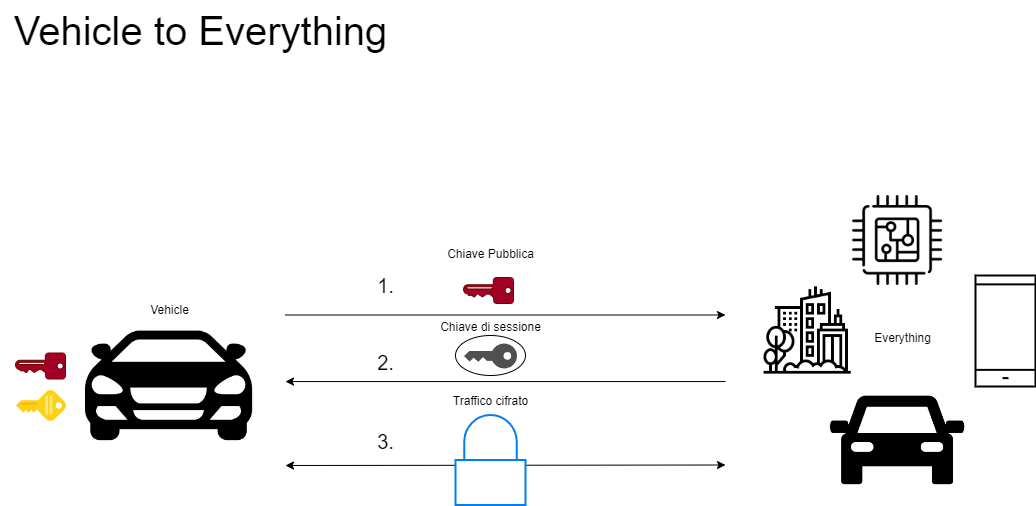
\includegraphics[width=0.7\textwidth]{capitoli/figure-conclusioni/v2x.png}
	\caption{Schema del protocollo in un contesto \textbf{V2X}}
	\label{fig:v2x}
\end{figure}

Tuttavia, in un contesto del genere, risulterebbe molto semplice per un attaccante ottenere informazioni sensibili o inviare informazioni false e errate semplicemente effettuando lo scambio e fingendosi qualcun'altro. Per tentare di ovviare a questo problema, si potrebbe prevedere un'autorità di certificazione che autentichi e certifichi ogni chiave pubblica che viene scambiata, come mostrato in \autoref{fig:v2x-ca}.

\begin{figure}[h]
	\centering
	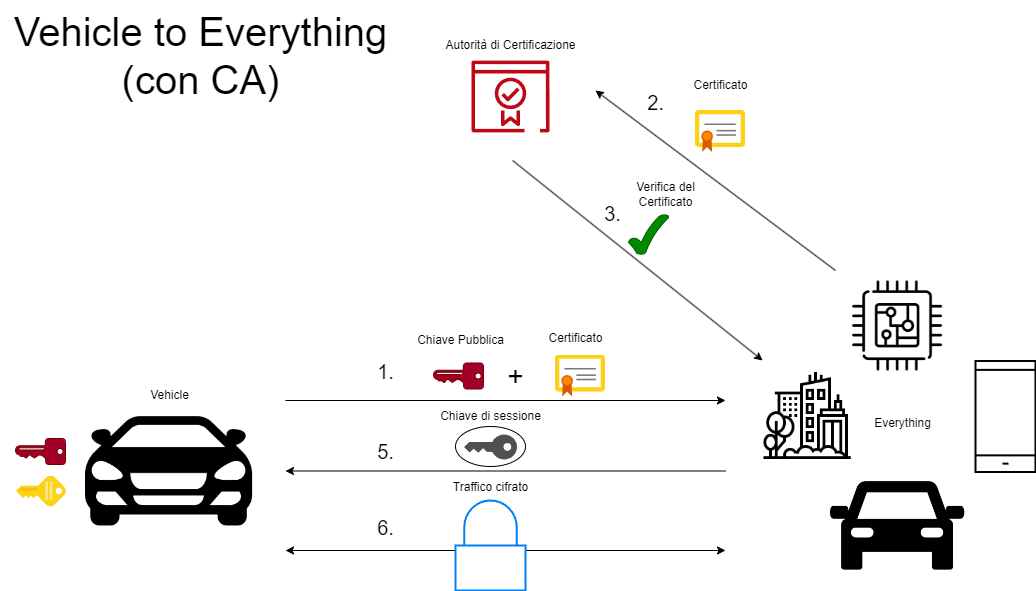
\includegraphics[width=0.7\textwidth]{capitoli/figure-conclusioni/v2x-ca.png}
	\caption{Schema del protocollo in un contesto \textbf{V2X} con \emph{CA}}
	\label{fig:v2x-ca}
\end{figure}

In questo modo, rilasciando dei certificati per ogni dispositivo nessuno può impersonare qualcun'altro e un attacco da parte di un malintenzionato diventa più difficile. Ma per effettuare tutte queste operazioni, purtroppo, è necessaria molta potenza di calcolo e molto tempo, quindi bisogna ottimizzare il protocollo per stringere i tempi e utilizzare dei processori che permettano una verifica dei protocolli più veloce.

\subsection{Aggiunta di un'autorità di certificazione}
La soluzione si è focalizzata principalmente sul problema della protezione del payload, tuttavia, questa può essere adattata anche al problema dell'\textbf{autenticazione} facendo alcuni accorgimenti.\\
Il problema principale di \emph{CAN} è che chiunque si collega alla rete è in grado di ricevere e trasmettere come il resto dei nodi, per cui è necessario un \emph{filtro} con cui stabilire chi può essere in grado di comunicare sulla rete. Riguardo la ricezione, per come è stato realizzato \emph{CAN}, non si può evitare ad un malintenzionato di mettersi in ascolto ma si possono proteggere i messaggi con la cifratura in modo tale da non esporre informazioni sensibili, mentre riguardo l'invio si può fare in modo che tutti i nodi \textbf{legittimi} ignorino ogni messaggio proveniente da un nodo non autorizzato. Per poter realizzare un sistema del genere bisognerebbe fare due modifiche:
\begin{itemize}
	\item Evitare di generare una coppia di chiavi ad ogni avvio, ma generarla solo la prima volta ed utilizzare quella. Questo non riduce la sicurezza del sistema realizzato ma bisogna fare attenzione alla segretezza delle \textbf{chiavi private}, poichè in caso di compromissione bisogna rigenerarle \textbf{immediatamente}.
	\item Prevedere la presenza di un nodo \emph{CA} che aiuti la rete a distinguere le chiavi pubbliche \textbf{autorizzate e non}, come mostrato in \autoref{fig:can-ca}
\end{itemize}

\begin{figure}[h]
	\centering
	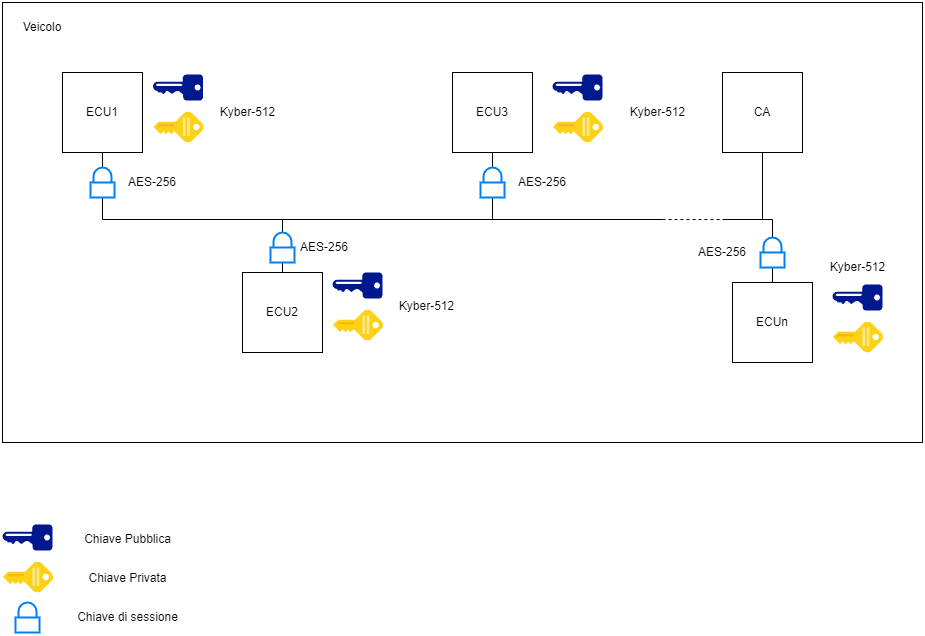
\includegraphics[width=0.6\textwidth]{capitoli/figure-conclusioni/can-ca.png}
	\caption{Rete \emph{CAN} con protezione del payload e nodo \emph{CA}}
	\label{fig:can-ca}
\end{figure}

In questo modo, si potrebbe modificare il protocollo in modo tale che, alla ricezione di una chiave pubblica, si attenda un riscontro positivo o negativo da parte del nodo \emph{CA} e, in base a questo, salvare o scartare la chiave ricevuta (oltre al traffico che proviene da quel nodo).

Ovviamente, oltre alla modifica al protocollo, bisognerebbe anche trovare un modo per garantire la provenienza dei riscontri da parte della \emph{CA}, poichè un nodo malizioso potrebbe generarsi da solo un riscontro positivo e inviarlo spacciandosi per il nodo \emph{CA}. In questo caso, un modo per garantire la provenienza del riscontro può essere quello di prevedere la presenza di una \textbf{firma}, ottenuta utilizzando uno schema di \textbf{firma digitale Post-Quantum} come \textbf{Dilithium}, anch'esso costruito su un problema basato sul \textbf{problema dei reticoli}. Tuttavia, oltre a dover necessariamente generare più messaggi per inviare sia riscontro che firma, si rischia di introdurre un onere computazionale troppo grande per l'hardware limitato di una \emph{ECU} e anche un ulteriore ritardo che rischia di compromettere la funzionalità di \emph{CAN}.
\newpage
